\section{Data}
% Describe how you explored your data, and the process through which you determined your
% input features. How did you end up representing your data? What else did you try? We are looking for:
% – A thorough exploration of the data, similar to what is presented in labs. What are the distributions of the features? How do these features correlate with the target?


% – If you use figures to answer those questions, an explanation of how you are interpreting those figures. Take care that your figures can be interpreted meaningfully.

% – A clear and logical description of how you determined your input features, with convincing logical or empirical evidence justifying your choice. Important features are not overlooked (e.g., not removed for “ease”).
% – A clear description of the way(s) that you are representing the data in your models.
% – The descriptions should be consistent with the .py and/or .ipynb files that you used while developing your model.
% – A clear description of how you are splitting your data into various sets. You may use k-fold cross validation if you’d like, but if you do, describe how you are applying that idea.


We used histograms and boxplots to explore the data depending on the data type.

% For numerical features such as Q1: How complex is it to make the food Q4: How much would you pay for the food, 
% we used box plots and histograms to see the distribution of data for each food class. Using boxplots allowed us to 
% identify the median and outliers of the responses and to see whether some food correlates with the question more than others. 

% id,"Q1: From a scale 1 to 5, how complex is it to make this food? (Where 1 is the most simple, and 5 is the most complex)",Q2: How many ingredients would you expect this food item to contain?,Q3: In what setting would you expect this food to be served? Please check all that apply,Q4: How much would you expect to pay for one serving of this food item?,Q5: What movie do you think of when thinking of this food item?,Q6: What drink would you pair with this food item?,"Q7: When you think about this food item, who does it remind you of?",Q8: How much hot sauce would you add to this food item?,Label


Figure \ref{f:hist_q1} shows a histogram of responses for Q1: From a scale 1 to 5, how complex is it to make this food?. For Sushi, 
the difficulty is generally higher with more inputs of 4 and 5. For Pizza, we see medium complexity(3) being the highest choice. For Shwa


\begin{figure}[h]
    \centerline{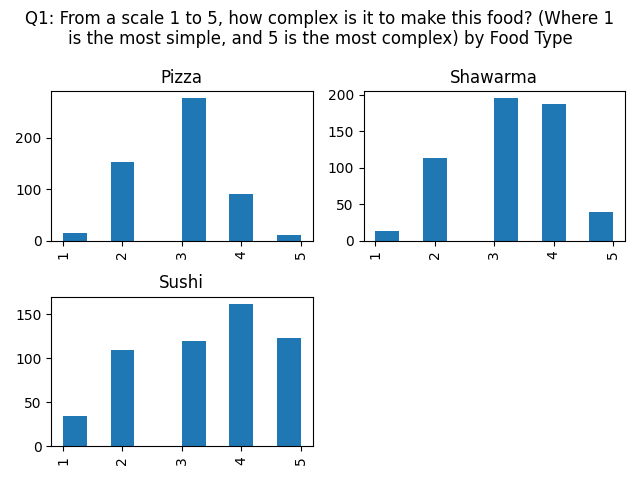
\includegraphics[width=\columnwidth]{data/histogram_Q1}}
    \caption{Histogram for Q1 How complex is it to make the food}
    \label{f:hist_q1}
\end{figure}

We see an interesting correlation between the number of ingredients and the food. For pizza, we have a normal 
distribution where the majority of the inputs labeled it as having a difficulty of 3. For sushi on the other hand, 
the distribution is more uniformed, with a peak of 4 but a wider spread.

For “how many ingredients would you expect this food item to contain”, we see the following plots showing a right skewed distribution for all food items.
For “How much would you expect to pay for one serving of this item”, we see the median for pizza is lower than sushi, and we see 
sushi with more extreme outliers than the other food classes.

We used bar charts for categorical data and only explored the questions with interesting data here. Some questions allowed open-ended answers, 
such as what movie associates with the food class. To make analysis simpler, we only plotted the top 5 most popular responses.
The following figure shows the results for Q5: What movie do you think of when thinking of this food item?. For both Pizza and Sushi, we saw 
“none” as the most popular input, and interestingly we saw “Avengers” to be by far the most popular response for Shawarma, suggesting a correlation 
between Avengers and Shawarma.

For Q3: “In what setting would you expect this food to be served?”, we see a trend that Pizza is more appropriate for most situations, and shawarma and sushi are more specific in when they are expected to be served.


Although there are other features such as Q7: “when you think about this food item, who does this remind you of?”, they show less differences for different food classes. For example, the most popular answer for Q7 was “Friends”, making it less indicative of the food class.

We split the dataset into 3 sets: 60\% training, 20\% validation and 20\% test. This allowed us sufficient data to train the model as well as data for testing that the models generalizes to unseen data



\begin{figure}[t!]
    \centerline{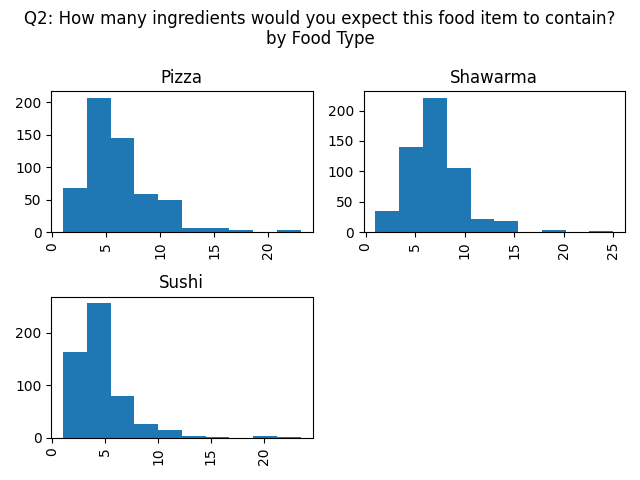
\includegraphics[width=\columnwidth]{data/histogram_Q2.png}}
    \caption{Histogram for Q2}
    \label{f:hist_q2}
\end{figure}

\begin{figure}[t!]
    \centerline{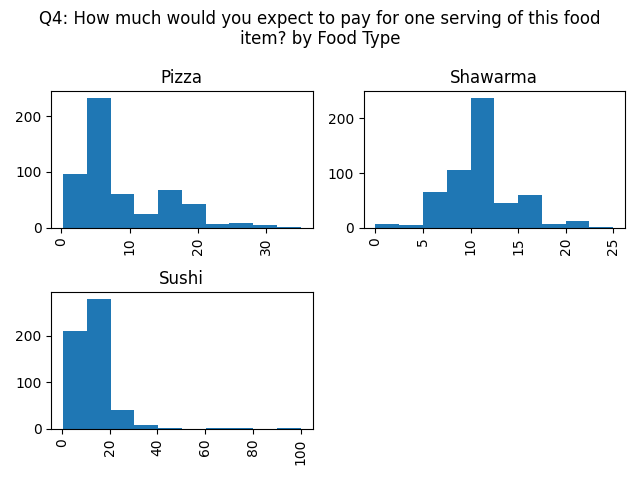
\includegraphics[width=\columnwidth]{data/histogram_Q4.png}}
    \caption{Histogram for Q4}
    \label{f:hist_q3}
\end{figure}